\documentclass[12pt]{article}
\usepackage[pdftex]{graphicx}
% \usepackage[numbers]{natbib}
\usepackage{natbib}
\usepackage{color}
\usepackage{amsmath}
\usepackage{amssymb}
\usepackage{verbatim}
\usepackage{mathpazo}
\usepackage{setspace}
\usepackage{multirow}
\usepackage{fullpage}
\usepackage{lscape}
\usepackage{array}
\usepackage{paralist}
\usepackage{fancyhdr}
\usepackage{graphicx}
\usepackage{makecell}
\usepackage{longtable}
\usepackage{xr}
\usepackage{subfig}
\externaldocument{ms}

\parindent=2em
\setlength{\parskip}{1ex}

\RequirePackage{lineno}

\begin{document}

\doublespacing
\linenumbers

%% reset counters for the SI \clearpage
\renewcommand{\thesection}{S\arabic{section}} \setcounter{section}{0}
\renewcommand{\theequation}{S\arabic{equation}}
\setcounter{equation}{0} \renewcommand{\thetable}{S\arabic{table}}
\setcounter{table}{0} % reset counter
\renewcommand{\thefigure}{S\arabic{figure}} \setcounter{figure}{0}
\setcounter{page}{1}

\newcommand{\lkmcomment}[1] {
  \textcolor{red}{\it{[#1]}}
}

% \begin{center} {\LARGE\textbf{Supplementary Information}}
% \end{center}

\begin{table}
  \renewcommand*\arraystretch{1.25}
  \centering
  \caption{Number of samples per year at each assembling hedgerow site. Asterisks indicate
    the year of planting for each restoration site. Sampling was not
    conducted in 2010 because resources were allocated to other
    projects.} 
  \begin{tabular}{lllllllllll}
    \hline
    \multicolumn{10}{c}{\hspace{10em}Year}\\
    & Site & 2006 & 2007 & 2008 & 2009 & 2010 & 2011 & 2012 & 2013 & 2014\\
    \hline
    % \multirow{5}{*}{\thead{Assembling \\ Hedgerows}}
    &HR1 & 4 & 3* & 3 & 3 & - & 3 & 4 & 5 & 3 \\ 
    &HR2 & 2 & 3 & 3* & 3 & - & 3 & 4 & 5 & 3 \\
    &HR3 & 2 & 3* & 3 & 3 & - & 3 & 4 & 5 & 3 \\
    &HR4 & - & 3 & 3* & 3 & - & 3 & 4 & 5 & 3 \\
    &HR5 & - & 3 & 3* & 3 & - & 3 & 4 & 5 & 3 \\
    \hline
  \end{tabular}
  \label{tab:maturing}
\end{table}
\clearpage

\begin{table}
  \renewcommand*\arraystretch{1.25}
  \centering
  \caption{Number of samples per year at each non-assembling hedgerow
    site. Asterisks indicate the site was sampled five or more times
    and thus included in the change point analysis.} 
  \begin{tabular}{lllllllllll}
    \hline
    \multicolumn{10}{c}{\hspace{10em}Year}\\
    & Site & 2006 & 2007 & 2008 & 2009 & 2010 & 2011 & 2012 & 2013 & 2014\\
    \hline
    % \multirow{19}{*}{\thead{Non-assembling \\ Hedgerows}}
    &HR6* & - & - & 1 & 4 & 4 & 2 & 4 & 5 & 3\\
    &HR7* & - & - & - & - & 4 & 2 & 6 & 5 & 3\\
    &HR8* & - & - & - & 3 & - & 2 & 4 & 5 & 3\\
    &HR9* & - & - & - & 4 & 4 & 2 & 4 & 5 & 3\\
    &HR10* & - & - & - & 4 & - & 1 & 4 & 5 & 3\\
    &HR11 & - & - & - & - & 4 & - & - & - & - \\
    &HR12 & - & - & - & - & - & - & 3 & 5 & 3\\
    &HR13 & 4 & - & - & - & - & - & - & - & -\\
    &HR14 & 4 & - & 1 & - & - & - & - & - & -\\
    &HR15 & - & - & - & - & - & - & 3 & 5 & 3\\
    &HR16 & - & - & - & - & - & - & 4 & 5 & 3\\
    &HR17 & - & - & - & - & - & - & 4 & 5 & 3\\
    &HR18 & - & - & - & - & - & - & 4 & 4 & 2 \\
    &HR19 & - & - & - & - & - & - & - & 5 & 3 \\
    &HR20 & - & - & - & - & - & - & 4 & 5 & 3\\
    &HR21 & - & - & - & - & - & - & 4 & 5 & -\\
    &HR22 & - & - & - & - & - & - & 4 & 5 & 3\\
    &HR23 & - & - & - & - & - & - & 4 & 5 & 3 \\
    &HR24 & - & - & - & - & - & - & 4 & - & -\\
    \hline
  \end{tabular}
  \label{tab:mature}
\end{table}
\clearpage

\begin{table}
  \renewcommand*\arraystretch{1.25}
  \centering
  \caption{Number of samples per year at each non-assembling field
    margin site. Asterisks indicate the site was sampled five or more times
    and thus included in the change point analysis.} 
  \begin{tabular}{lllllllllll}
    \hline
    \multicolumn{10}{c}{\hspace{10em}Year}\\
    & Site & 2006 & 2007 & 2008 & 2009 & 2010 & 2011 & 2012 & 2013 & 2014\\
    \hline
    % \multirow{29}{*}{\thead{Non-assembling \\ field margins}}
    &FM1* & 4 & 3 & 3 & 3 & - & 3 & 4 & 5 & 3\\
    &FM2* & 4 & 3 & 3 & 3 & - & 3 & 4 & 5 & 3\\
    &FM3* & - & - & - & 3 & 4 & - & 3 & 5 & 3\\
    &FM4 & 4 & 3 & 3 & - & - & - & - & - & -\\
    &FM5* & - & 3 & 3 & 3 & - & 3 & 4 & 4 & 3\\
    &FM6 & - & - & - & - & - & - & 3 & 4 & 2\\
    &FM7* & - & 3 & 3 & 3 & - & 2 & 4 & 4 & 2\\
    &FM8 & - & - & - & 4 & - & - & 4 & 5 & 3\\
    &FM9 & - & - & - & - & - & - & 1 & 5 & 2\\
    &FM10 & 4 & - & - & - & - & - & - & - & -\\
    &FM11 & 4 & - & - & - & - & - & - & - & -\\
    &FM12* & - & 3 & 3 & 3 & - & 3 & 4 & 5 & 3\\
    &FM13* & 4 & 3 & 3 & 3 & - & 3 & 3 & 5 & 3\\
    &FM14 & - & - & - & 4 & - & - & 3 & 3 & 1\\
    &FM15 & - & - & - & - & - & - & 3 & - & -\\
    &FM16 & - & 3 & 3 & 3 & - & 3 & - & - & -\\
    &FM17* & - & - & - & 4 & 4 & - & 3 & 5 & 1\\
    &FM18 & - & - & - & - & 4 & - & - & - & -\\
    &FM19 & - & - & - & - & - & - & - & 5 & 3\\
    &FM20 & - & - & - & - & - & - & - & 5 & 3\\
    &FM21 & - & - & - & - & - & - & 3 & - & -\\
    &FM22* & - & 3 & 3 & 3 & - & 3 & 4 & 3 & 1\\
    &FM23 & 4 & - & - & - & - & - & - & - & -\\
    &FM24 & - & - & - & - & - & - & - & 1 & -\\
    &FM25 & - & - & - & - & - & - & 3 & 5 & 3\\
    &FM26* & - & 3 & 3 & 3 & - & 3 & 2 & 4 & 2\\
    &FM27* & 4 & 3 & 3 & 3 & - & 3 & 4 & 4 & 2\\
    &FM28 & - & - & - & - & - & - & 4 & 5 & 2\\
    &FM29 & - & - & - & - & 4 & - & 5 & 4 & 3\\
    \hline
  \end{tabular}
  \label{tab:controls}
\end{table}
\clearpage


\begin{figure}[!tbp]
  \centering
  \subfloat[]{\includegraphics[width=0.48\textwidth]{figures/before.pdf}\label{fig:f1}}
  \hfill
  \subfloat[]{\includegraphics[width=0.48\textwidth]{figures/after.pdf}\label{fig:f2}}
  \caption{Photographs of on of the restoration sites. (a) immediately prior to its restoration and (b) post-restoration.}
\end{figure}
\clearpage


\begin{figure}
  \centering
  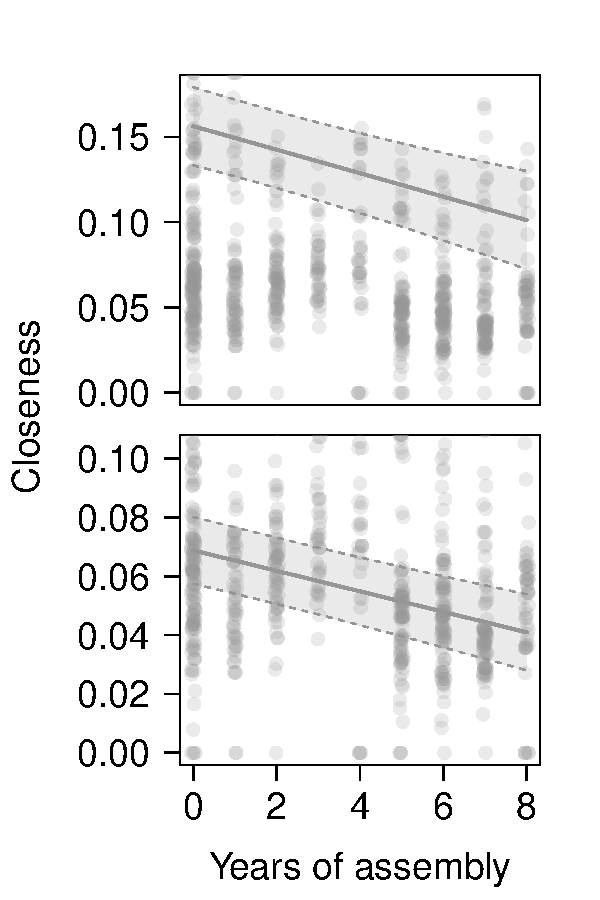
\includegraphics[width=.6\textwidth]{../analysis/speciesLevel/figures/closenessPanel.pdf}
  \caption{The closeness of pollinators and plants decreased slightly
    through time. Points represent means for each species across
    sites. The solid line indicates the mean slope estimate and the
    dashed lines are the $95\%$ confidence intervals around the
    estimate.}
  \label{fig:closeness}
\end{figure}
\clearpage


\end{document}

%%% Local Variables:
%%% mode: latex
%%% TeX-PDF-mode: t
%%% End:
